	
From the Fig. \ref{fig:4.1.5_qseventeen} we obtain the coordinates as,
\begin{align}
\vec{O} = \myvec{0\\0} \quad\vec{A} = \myvec{0.707\\0.707} \quad\vec{B} = \myvec{0.707\\0} \quad\vec{C} = \myvec{1\\0} 
\end{align}
 The required area is the sector $OAC$.  This is given by
\begin{align}
ar\brak{OACB} &= ar\brak{OAB} + ar\brak{BAC}
\\
ar\brak{BAC} &= \frac{1}{2}\norm{\brak{\vec{B-A}}\times\brak{\vec{C-A}}}
\\
ar\brak{OAB} &= \frac{1}{2}\norm{\brak{\vec{B-O}}\times\brak{\vec{A-O}}}
\end{align}
which on computing, we obtain the required area as 0.3535
\begin{comment}
\begin{align}
\cos{\angle{BOA}} = \frac{\norm{\vec{OA}}^2 + \norm{\vec{OB}}^2 - \norm{\vec{AB}}^2}{2\norm{\vec{OA}}\norm{\vec{OB}}}
\\
\cos{\angle{BOA}} = \frac{1}{\sqrt{2}}
\\
\implies \angle{BOA} = 45\degree
\end{align}
 The required area is given by
\begin{align}
ar\brak{OACB} = \frac{\angle{BOA}}{360} \times \pi \times 1^2
\end{align}
\end{comment}
\begin{comment}
\begin{align} 
ar\brak{OACB} = ar\brak{OAB} + ar\brak{ACB}\\
ar\brak{OACB} = \int\limits_{0}^{0.707} x dx + \int\limits_{0.707}^{1} \sqrt{1-x^2}dx
\end{align}
\end{comment}

The following python code computes the required area represented in Fig.\ref{fig:4.1.5_qseventeen}.
	\begin{lstlisting}
	./solutions/5/codes/circle/q17ag.py
	\end{lstlisting}
\begin{figure}[!ht]
	\centering
	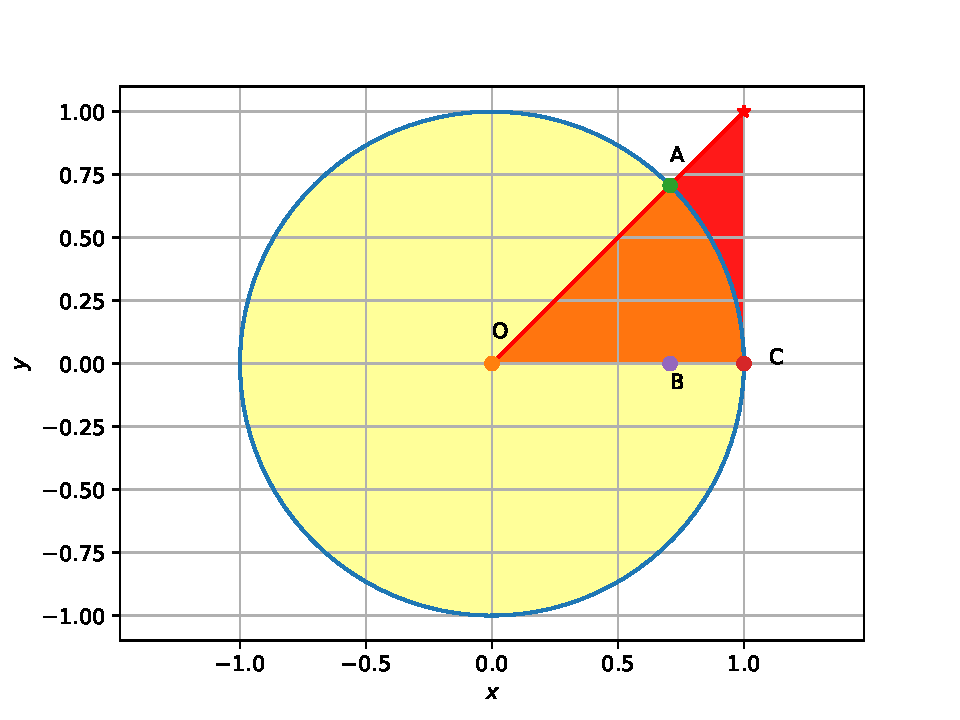
\includegraphics[width=\columnwidth]{./solutions/5/figs/circle/q17.eps}
	\caption{}
	\label{fig:4.1.5_qseventeen}	
	\end{figure}
	
\end{enumerate}
